\pdfbookmark{Общая характеристика работы}{characteristic}             % Закладка pdf
\section*{Общая характеристика работы}

\newcommand{\actuality}{\pdfbookmark[1]{Актуальность}{actuality}\underline{\textbf{\actualityTXT}}}
\newcommand{\progress}{\pdfbookmark[1]{Разработанность темы}{progress}\underline{\textbf{\progressTXT}}}
\newcommand{\aim}{\pdfbookmark[1]{Цели}{aim}\underline{{\textbf\aimTXT}}}
\newcommand{\tasks}{\pdfbookmark[1]{Задачи}{tasks}\underline{\textbf{\tasksTXT}}}
\newcommand{\aimtasks}{\pdfbookmark[1]{Цели и задачи}{aimtasks}\aimtasksTXT}
\newcommand{\novelty}{\pdfbookmark[1]{Научная новизна}{novelty}\underline{\textbf{\noveltyTXT}}}
\newcommand{\influence}{\pdfbookmark[1]{Практическая значимость}{influence}\underline{\textbf{\influenceTXT}}}
\newcommand{\methods}{\pdfbookmark[1]{Методология и методы исследования}{methods}\underline{\textbf{\methodsTXT}}}
\newcommand{\defpositions}{\pdfbookmark[1]{Положения, выносимые на защиту}{defpositions}\underline{\textbf{\defpositionsTXT}}}
\newcommand{\reliability}{\pdfbookmark[1]{Достоверность}{reliability}\underline{\textbf{\reliabilityTXT}}}
\newcommand{\probation}{\pdfbookmark[1]{Апробация}{probation}\underline{\textbf{\probationTXT}}}
\newcommand{\contribution}{\pdfbookmark[1]{Личный вклад}{contribution}\underline{\textbf{\contributionTXT}}}
\newcommand{\publications}{\pdfbookmark[1]{Публикации}{publications}\underline{\textbf{\publicationsTXT}}}


{\actuality} В условиях растущего мирового населения и активной глобальной индустриализации, сопровождаемых повышением объемов потребления электроэнергии,
все более актуальной становится \fixme{разработка новых подходов и источников энергии}, способных обеспечить устойчивое и надежное энергоснабжение. \fixme{Необходимость в этом также обуславливается стремлением к эффективному использованию природных ресурсов и минимизации негативного воздействия на окружающую среду.} Одним из наиболее перспективных направлений является управляемый термоядерный синтез (УТС), рассматриваемый в качестве \fixme{<<чистой>> альтернативы традиционным подходам на основе сжигания ископаемых ресурсов, так и ключевого звена гибридной системы в реакторах типа синтез-деление.} Прогресс в области УТС может стать ключевым фактором в развитии энергетических технологий следующего поколения.

За последние десятилетия наибольшие успехи на пути к практической реализации контролируемой реакции УТС были достигнуты в установках с магнитным удержанием горячей плазмы типа токамак. Возможность \fixme{горения} дейтерий-тритиевой (DT) реакции термоядерного синтеза была продемонстрирована на токамаках TFTR~\cite{Skinner1997} и JET~\cite{Keilhacker1999} еще в конце XX века. Последующая модернизация токамака JET и оптимизация методики эксперимента позволила достичь \fixme{на сегодняшний день рекордных параметров DT-плазмы с протекающей реакцией синтеза и длительностью разряда около \SI{6}{\second}}~\cite{Maggi2024,Kappatou2025}. На токамаках WEST и EAST были получены рекордные результаты по длительности удержания горячей плазмы (без генерации термоядерной энергии) продолжительностью в \(\SI{364}{\second}\)~\cite{Shi2025} и \(\SI{1056}{\second}\)~\cite{Gong2024}, соответственно. Наблюдаемые достижения свидетельствует о перспективности и потенциальной реализуемости УТС за счет удержания термоядерной плазмы в магнитной конфигурации токамака.

В настоящее время идет активная фаза строительства международного экспериментального термоядерного реактора ИТЭР, спроектированного для практической демонстрации возможности \fixme{длительного (\SI{400}{\second})} удержания термоядерной DT-плазмы и решения сопутствующих инженерных задач. Введены в эксплуатацию наибольший в России токамак Т15-МД~\cite{Velikhov2024} и наибольший в мире токамак JT60-SA~\cite{Shirai2024}, расположенный в Японии. Во множестве стран разрабатываются проекты установок следующего поколения для отработки реакторных технологий, в том числе в России ведется активное проектирование токамака с реакторными технологиями (ТРТ)~\cite{Krasilnikov2021}. Помимо этого, растет число частных компаний в области УТС, развивающих уникальные подходы и технологии для коммерческих целей. По данным Ассоциации термоядерной промышленности (FIA)~\cite{FIA}, более 50\% компаний из данной сферы разрабатывают подходы на основе магнитного удержания плазмы, что дополнительно подчеркивает актуальность направления.

Ввод в эксплуатацию термоядерных установок (ТЯУ) потребует решения целого ряда физических и технологических задач. Одними из наиболее существенных остаются проблемы удержания энергии и частиц, выбора материалов обращенных к плазме элементов (ОПЭ), эффективной организации топливного цикла, а также обеспечения радиационной безопасности. Последний пункт обусловлен планируемым использованием смеси дейтерия и радиоактивного трития в качестве топлива для термоядерных реакторов, что определяет необходимость в понимании процессов накопления и систематическом контроле содержания изотопов водорода в конструкционных элементах.

В первых экспериментах с DT-плазмой на токамаках TFTR и JET наблюдалось чрезмерно большое накопление трития~\cite{Gasparyan2024}, связанное с особенностями взаимодействия изотопов водорода с используемыми на тот момент углеродными ОПЭ. Последующие результаты, полученные на токамаках с металлической облицовкой (JET~\cite{Maggi2024,Kappatou2025}: бериллиевая первая стенка и вольфрамовый дивертор; ASDEX-Upgrade~\cite{Rohde2009}: вольфрамовые первая стенка и дивертор), продемонстрировали перспективу в достижении \fixme{соизмеримых} параметров удержания плазмы при одновременном снижении (по сравнению с углеродными ОПЭ) скорости накопления изотопов водорода более чем на порядок. Важно заметить, что вольфрам используется в качестве основного материала наиболее нагруженной области большинства действующих токамаков "--- дивертора. Как материал ОПЭ, вольфрам характеризуется низким коэффициентом распыления легкими ионами и высокой температуростойкости, что может играть ключевую роль в обеспечении продолжительного срока службы под воздействием интенсивных нейтронных и плазменных потоков~\cite{Neu2005}. К тому же, Международной организацией ИТЭР было принято решение о переходе к полностью вольфрамовой облицовке~\cite{Barabaschi2025}, а во множестве проектов демонстрационных реакторов вольфрам рассматривается как приоритетный материал ОПЭ~\cite{Bachmann2016}.

Оценки уровня накопленного трития в ИТЭР~\cite{Roth1,Pitts2025} с полностью вольфрамовой стенкой показывают, что допустимый уровень содержания не должен быть превышен за период эксплуатации. Однако при получении данных консервативных оценок не учитывался ряд процессов, протекание которых ожидается во время работы реактора. Одним из таких факторов являются быстрые переходные процессы, как локализованные на периферии неустойчивости (ELMs "--- Edge localised modes), наблюдаемые в режимах с наилучшими параметрами удержания плазмы в токамаках (H-мода). Развитие ELM-неустойчивости сопровождается \fixme{мощными кратковременными ($\leq\SI{1}{\milli\second}$) потоками тепла и высокоэнергетичных частиц, приходящими на ОПЭ с характерной частотой \(\sim \SIrange{10}{100}{\hertz}\)}. Длительное импульсно-периодическое воздействие плазменных потоков может влиять как на динамику накопления рабочего газа в ОПЭ, так и на процессы взаимодействия плазмы с их поверхностью.

\fixme{Немногочисленные эксперименты по имитации воздействия мощных плазменных потоков, соответствующих ELM-событиям, на захват изотопов водорода в вольфраме проводились на линейных плазменных установках~\cite{Nishijima2011,Poskakalov2020,Ogorodnikova}. Полученные результаты указывают на потенциально большую скорость проникновения изотопов водорода вглубь материала при импульсном воздействии по сравнению со случаем стационарного облучения, характерного для нормальных плазменных разрядов, однако не дают однозначной информации о влиянии на скорость интегрального накопления. Помимо этого, параметры облучения в установках такого типа не могут в полной мере воспроизвести условия, соответствующие крупным токамакам масштаба ИТЭР. Численное моделирование длительного накопления на больших временных масштабах также затруднительно ввиду малой длительности переходных процессов. }

\fixme{Диагностика содержания изотопов водородов в ОПЭ является не менее приоритетным вопросом. В настоящее время особое внимание уделяется развитию методов дистанционного контроля, основанных на использовании лазерного излучения. Одним из таких методов является лазерно-индуцированная десорбция (ЛИД), которая основана на нагреве участка исследуемой поверхности лазерным импульсом с последующим анализом состава вышедшего газа. Применимость ЛИД была продемонстрирована на \fixme{ряде} установок (TEXTOR~\cite{Schweer2009}, JET~\cite{Zlobinski2024}, Глобус-М2~\cite{Medvedev2024} и т.д.), а соответствующие диагностические комплексы разрабатываются для ИТЭР и были предложены для российского проекта ТРТ~\cite{Razdobarin2022}. Выход изотопов водорода из ОПЭ под действием импульсных тепловых нагрузок является схожим и в то же время более простым процессом по сравнению со случаем захвата при импульсно-периодическом плазменном облучении. Тем не менее, исследование основных зависимостей выхода при лазерном нагреве является актуальным вопросом для определения наиболее эффективных режимов диагностического метода.}

{\aim} диссертационной работы является выявление закономерностей процессов удержания и выхода дейтерия в вольфраме при импульсном плазменном и лазерном воздействии.

Для~достижения поставленной цели необходимо было решить следующие~{\tasks}:
\begin{enumerate}[beginpenalty=10000] % https://tex.stackexchange.com/a/476052/104425
    \item \fixme{Построить математическую модель, описывающую транспорт дейтерия в вольфраме под действием импульсных тепловых и плазменных нагрузок.}
    \item \fixme{Провести анализ применимости стандартных моделей транспорта изотопов водорода в материалах к моделированию процессов захвата и десорбции при импульсных нагрузках.}
    \item Оценить параметры плазменных нагрузок, приходящих на ОПЭ во время ELM-событий, \fixme{на основе данных для ИТЭР.}
    \item Исследовать влияние быстрых переходных процессов, соответствующих ELM-событиям, \fixme{на накопление дейтерия в вольфраме на временных масштабах, соответствующих длительности плазменных разрядов в ИТЭР.}
    \item Провести анализ состава потока десорбированного дейтерия с поверхности вольфрама при лазерном нагреве.
    \item \fixme{Определить влияние процессов на поверхности, параметров центров захвата, теплофизических свойств материала и характеристик импульса на выход дейтерия из вольфрама при лазерном нагреве.}
\end{enumerate}

{\methods} Достижение поставленной цели и решение сопутствующих задач осуществлялись путем проведения численного моделирования, которое позволяет исследовать влияние импульсных нагрузок в широком диапазоне параметров, обычно недоступном в рамках действующих экспериментальных и лабораторных установок. Результаты численных расчетов были получены методом конечных элементов в свободно распространяемом программном пакете \href{https://github.com/festim-dev/FESTIM}{FESTIM}, разработанном в международном коллективе при участии автора. Для решения части ресурсоёмких задач были использованы мощности высокопроизводительного вычислительного центра \thesisOrganizationShort. Для демонстрации надежности и корректности использованных моделей проводилась их верификация и валидация путем сравнения с экспериментальными результатами. Построение аналитической модели, описывающей распределение изотопов водорода в вольфраме при наличии центров захвата изотопов водорода и градиента температур (эффект Соре), проводилось путем решения системы дифференциальных уравнений в частных производных методом функции Грина.

{\novelty}
\begin{enumerate}[beginpenalty=10000] % https://tex.stackexchange.com/a/476052/104425
    \item \fixme{Впервые проведено моделирование длительного (\SI{1000}{\second}) накопления дейтерия в вольфрамовых ОПЭ под действием импульсно-периодических плазменных нагрузок, соответствующих ELM-событиям в крупных токамаках, с длительностью одного события \SI{1}{\milli\second} и частотой повторения от \num{10} до \SI{100}{\hertz} (от \num{e4} до \num{e5} событий)}.
    \item \fixme{Предложена оригинальная аналитическая модель, описывающая одномерное стационарное распределение содержания водорода в материалах при наличии центров захвата и градиента температур в приближении мгновенной рекомбинации атомов на обращенной к плазме поверхности и мгновенной рекомбинации или нулевого потока атомов на обратной поверхности.}
    \item Впервые проведен детальный анализ состава потока дейтерия, десорбированного с поверхности вольфрама при лазерном нагреве.
    \item \fixme{Впервые проведена оценка роли процессов на поверхности, центров захвата, теплофизических свойств и параметров импульса на выход дейтерия из поверхностных слоев вольфрама при лазерном нагреве}.
\end{enumerate}

{\influence} заключается в следующем:
\begin{enumerate}[beginpenalty=10000] % https://tex.stackexchange.com/a/476052/104425
    \item \fixme{Результаты анализа влияния импульсно-периодических нагрузок на накопление изотопов водорода в вольфраме могут быть использованы \fixme{для прогноза} содержания изотопов водорода, накопленных в ОПЭ ТЯУ.}
    \item \fixme{Результаты анализа влияния параметров лазерного нагрева и материала на выход дейтерия из поверхностных слоев вольфрама} могут быть использованы при разработке и выборе оптимальных параметров диагностического метода контроля содержания изотопов водорода в ОПЭ, основанного на ЛИД. Результаты экспериментов по ЛИД дейтерия из соосажденных пленок вольфрама могут быть использованы для валидации численных моделей.
    \item Имплементированная в коде FESTIM модель, учитывающая поверхностные процессы, доступна всем пользователям кода и существенно расширяет его область применения. Результаты валидации модели включены в книгу по верификации и валидации кода FESTIM и могут быть использованы для проведения сравнения результатов, полученных с помощью иных кодов.
\end{enumerate}

{\defpositions}
\begin{enumerate}[beginpenalty=10000] % https://tex.stackexchange.com/a/476052/104425
    \item \fixme{Одномерная аналитическая модель, описывающая стационарное распределение водорода в материале при учете центров захвата и градиента температур, позволяет оценить предельное содержание изотопов водорода под действием импульсно-периодических плазменных нагрузок при достижении квазистационарного режима.}
    \item Возникновение импульсно-периодических плазменных нагрузок, соответствующих ELM-событиям в токамаках (частота: 10 "--- 100 Гц, длительность: \SI{1}{\milli\second}, плотность энергии: \SIrange{0.14}{0.45}{\mega\joule\per\meter\squared}), наряду со стационарными плазменными потоками (плотность мощности: \SIrange{1}{10}{\mega\watt\per\meter\squared}) ведет к снижению скорости накопления дейтерия в вольфраме при длительности облучения более \SI{10}{\second} за счет значительного повышения температуры материала относительно случая облучения стационарными потоками плазмы. 
    \item Дополнительный нагрев во время импульсно-периодических плазменных нагрузок, соответствующих ELM-событиям в токамаках, приводит к более быстрому проникновению дейтерия вглубь материала за счет большей подвижности, что может усложнить процесс обезгаживания ОПЭ в ТЯУ. 
    \item \fixme{Атомарная фракции в потоке дейтерия, десорбированного с поверхности вольфрама, растет с увеличением температуры поверхности и уменьшением потока частиц, выходящих на поверхность. Интегральная величина атомарной фракции в потоке десорбированного водорода может достигать $\sim$10~\% при лазерном нагреве с длительностью более \SI{10}{\micro\second} до температуры плавления вольфрама, что может вносить дополнительную погрешность измерений при анализа содержания изотопов водорода методом ЛИД.} 
    \item \fixme{Процессы на поверхности могут приводить к снижению доли десорбированного дейтерия из вольфрама при импульсном лазерном нагреве с длительностью менее \SI{10}{\micro\second}, уменьшая эффективность анализа содержания изотопов водорода в толстых поверхностных слоях методом ЛИД.}
\end{enumerate}

{\reliability} \fixme{полученных результатов обеспечивается применением общепризнанного численного метода решения систем дифференциальных уравнений в частных производных (метод конечных элементов), имплементированного в верифицированном и валидированном программном пакете FESTIM. Построение численных моделей проводилось на основе известных теорий, надежность которых была продемонстрирована путем воспроизведения результатов множества лабораторных экспериментов. Помимо этого, использованные модели были валидированы путем сравнения результатов численных расчетов с экспериментальными данными.} Полученные результаты демонстрируют качественное и количественное согласие с данными, полученными независимыми авторами на основе моделирования или экспериментального анализа.

{\probation}
Основные результаты работы докладывались и обсуждались на российских и международных конференциях:
\begin{itemize}
    \item XXV, XXVI, XXVII, XXVIII конференции <<Взаимодействие плазмы с поверхностью>> (Москва, 2022 "--- 2025 гг.);
    \item Пятнадцатая международная школа молодых ученых и специалистов им. А.А. Курдюмова (Окуловка, 2022 г.);
    \item XX Всероссийская конференция <<Диагностика высокотемпературной плазмы>> (Сочи, 2023 г.);
    \item 26th International Conference on Plasma Surface Interaction in Controlled Fusion Devices (Marseille, France, 2024 г.);
    \item 1st Open Source Software for Fusion Energy Conference (2025 г.).
\end{itemize}
Полученные результаты также представлялись и обсуждались на собраниях разработчиков программного пакета FESTIM. 

{\contribution} Все результаты, выносимые на защиту, были получены автором или при его непосредственном участии. Лично автором были построены численные и аналитические модели, использованные для исследования процессов накопления и выхода дейтерия из вольфрама под действием импульсных плазменных и лазерных нагрузок, проведены моделирование и обработка полученных результатов. Постановка задач, выбор входных параметров для моделирования и анализ полученных результатов обсуждались с непосредственным научным руководителем д.ф.-м.н. Ю.М. Гаспаряном. Имплементация модели, учитывающей поверхностные процессы, в коде FESTIM проводилась совместно с главным разработчиком кода Ph.D. Р. Делапорте-Матюран (MIT) при определяющем участии автора, реализовавшим модель и осуществившим ее верификацию и валидацию. Эксперименты по ЛИД дейтерия из соосажденных пленок вольфрама были проведены \fixme{научным коллективом ФТИ им. А.Ф. Иоффе} при непосредственном участии автора в постановке экспериментов, обработке результатов измерений и проведении сравнения с модельными данными.

\ifnumequal{\value{bibliosel}}{0}
{%%% Встроенная реализация с загрузкой файла через движок bibtex8. (При желании, внутри можно использовать обычные ссылки, наподобие `\cite{vakbib1,vakbib2}`).
    {\publications} Основные результаты по теме диссертации изложены
    в~XX~печатных изданиях,
    X из которых изданы в журналах, рекомендованных ВАК,
    X "--- в тезисах докладов.
}%
{%%% Реализация пакетом biblatex через движок biber
    \begin{refsection}[bl-author, bl-registered]
        % Это refsection=1.
        % Процитированные здесь работы:
        %  * подсчитываются, для автоматического составления фразы "Основные результаты ..."
        %  * попадают в авторскую библиографию, при usefootcite==0 и стиле `\insertbiblioauthor` или `\insertbiblioauthorgrouped`
        %  * нумеруются там в зависимости от порядка команд `\printbibliography` в этом разделе.
        %  * при использовании `\insertbiblioauthorgrouped`, порядок команд `\printbibliography` в нём должен быть тем же (см. biblio/biblatex.tex)
        %
        % Невидимый библиографический список для подсчёта количества публикаций:
        \phantom{\printbibliography[heading=nobibheading, section=1, env=countauthorvak,          keyword=biblioauthorvak]%
            \printbibliography[heading=nobibheading, section=1, env=countauthorwos,          keyword=biblioauthorwos]%
            \printbibliography[heading=nobibheading, section=1, env=countauthorscopus,       keyword=biblioauthorscopus]%
            \printbibliography[heading=nobibheading, section=1, env=countauthorconf,         keyword=biblioauthorconf]%
            \printbibliography[heading=nobibheading, section=1, env=countauthorother,        keyword=biblioauthorother]%
            \printbibliography[heading=nobibheading, section=1, env=countregistered,         keyword=biblioregistered]%
            \printbibliography[heading=nobibheading, section=1, env=countauthorpatent,       keyword=biblioauthorpatent]%
            \printbibliography[heading=nobibheading, section=1, env=countauthorprogram,      keyword=biblioauthorprogram]%
            \printbibliography[heading=nobibheading, section=1, env=countauthor,             keyword=biblioauthor]%
            \printbibliography[heading=nobibheading, section=1, env=countauthorvakscopuswos, filter=vakscopuswos]%
            \printbibliography[heading=nobibheading, section=1, env=countauthorscopuswos,    filter=scopuswos]}%
        %
        \nocite{*}%
        %
        {\publications} Основные результаты по теме диссертации опубликованы в~\arabic{citeauthor}~печатных работах,
        \ifnum \value{citeauthorvak}>0
            \arabic{citeauthorvak} из которых издана в рецензируемом журнале, включенном в перечень ВАК РФ%
        \fi
        \ifnum \value{citeauthorscopuswos}>0%
            которые изданы в~периодических научных журналах, индексируемых Web of~Science и Scopus
            и приравненных к журналам из перечня ВАК РФ%
        \fi%
        \ifnum \value{citeauthorconf}>0%
            , \arabic{citeauthorconf} "--- в~тезисах докладов.
        \else%
            .
        \fi%
        \ifnum \value{citeregistered}=1%
            \ifnum \value{citeauthorpatent}=1%
                Зарегистрирован \arabic{citeauthorpatent} патент.
            \fi%
            \ifnum \value{citeauthorprogram}=1%
                Зарегистрирована \arabic{citeauthorprogram} программа для ЭВМ.
            \fi%
        \fi%
        \ifnum \value{citeregistered}>1%
            Зарегистрированы\ %
            \ifnum \value{citeauthorpatent}>0%
                \formbytotal{citeauthorpatent}{патент}{}{а}{}%
                \ifnum \value{citeauthorprogram}=0 . \else \ и~\fi%
            \fi%
            \ifnum \value{citeauthorprogram}>0%
                \formbytotal{citeauthorprogram}{программ}{а}{ы}{} для ЭВМ.
            \fi%
        \fi%
        % К публикациям, в которых излагаются основные научные результаты диссертации на соискание учёной
        % степени, в рецензируемых изданиях приравниваются патенты на изобретения, патенты (свидетельства) на
        % полезную модель, патенты на промышленный образец, патенты на селекционные достижения, свидетельства
        % на программу для электронных вычислительных машин, базу данных, топологию интегральных микросхем,
        % зарегистрированные в установленном порядке.(в ред. Постановления Правительства РФ от 21.04.2016 N 335)
    \end{refsection}%
    \begin{refsection}[bl-author, bl-registered]
        % Это refsection=2.
        % Процитированные здесь работы:
        %  * попадают в авторскую библиографию, при usefootcite==0 и стиле `\insertbiblioauthorimportant`.
        %  * ни на что не влияют в противном случае
    \end{refsection}%
    %
    % Всё, что вне этих двух refsection, это refsection=0,
    %  * для диссертации - это нормальные ссылки, попадающие в обычную библиографию
    %  * для автореферата:
    %     * при usefootcite==0, ссылка корректно сработает только для источника из `external.bib`. Для своих работ --- напечатает "[0]" (и даже Warning не вылезет).
    %     * при usefootcite==1, ссылка сработает нормально. В авторской библиографии будут только процитированные в refsection=0 работы.
}


 % Характеристика работы по структуре во введении и в автореферате не отличается (ГОСТ Р 7.0.11, пункты 5.3.1 и 9.2.1), потому её загружаем из одного и того же внешнего файла, предварительно задав форму выделения некоторым параметрам

%Диссертационная работа была выполнена при поддержке грантов \dots

%\underline{\textbf{Объем и структура работы.}} Диссертация состоит из~введения,
%четырех глав, заключения и~приложения. Полный объем диссертации
%\textbf{ХХХ}~страниц текста с~\textbf{ХХ}~рисунками и~5~таблицами. Список
%литературы содержит \textbf{ХХX}~наименование.

\pdfbookmark{Содержание работы}{description}                          % Закладка pdf
\section*{Содержание работы}
Во \underline{\textbf{введении}} обосновывается актуальность
исследований, проводимых в~рамках данной диссертационной работы,
приводится обзор научной литературы по~изучаемой проблеме,
формулируется цель, ставятся задачи работы, излагается научная новизна
и практическая значимость представляемой работы. В~последующих главах
сначала описывается общий принцип, позволяющий \dots, а~потом идёт
апробация на частных примерах: \dots  и~\dots.


\underline{\textbf{Первая глава}} посвящена \dots

картинку можно добавить так:
\begin{figure}[ht]
    \centerfloat{
        \hfill
        \subcaptionbox{\LaTeX}{%
            
\includegraphics[scale=0.27]{latex}}
        \hfill
        \subcaptionbox{Knuth}{%
            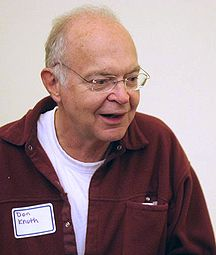
\includegraphics[width=0.25\linewidth]{knuth1}}
        \hfill
    }
    \caption{Подпись к картинке.}\label{fig:latex}
\end{figure}

Формулы в строку без номера добавляются так:
\[
    \lambda_{T_s} = K_x\frac{d{x}}{d{T_s}}, \qquad
    \lambda_{q_s} = K_x\frac{d{x}}{d{q_s}},
\]

\underline{\textbf{Вторая глава}} посвящена исследованию

\underline{\textbf{Третья глава}} посвящена исследованию

В \underline{\textbf{четвертой главе}} приведено описание

\FloatBarrier
\pdfbookmark{Заключение}{conclusion}                                  % Закладка pdf
В \underline{\textbf{заключении}} приведены основные результаты работы, которые заключаются в следующем:
%% Согласно ГОСТ Р 7.0.11-2011:
%% 5.3.3 В заключении диссертации излагают итоги выполненного исследования, рекомендации, перспективы дальнейшей разработки темы.
%% 9.2.3 В заключении автореферата диссертации излагают итоги данного исследования, рекомендации и перспективы дальнейшей разработки темы.
В рамках данной диссертационной работы методом численного моделирования были исследованы закономерности захвата и десорбции дейтерия в вольфраме при импульсных плазменном и лазерном воздействии. Среди наиболее значимых результатов можно выделить следующие:
\begin{enumerate}
  \item В программном пакете FESTIM была реализована модель, учитывающая кинетику процессов на поверхности. Реализованная модель расширяет функциональные возможности кода, что подтверждено в ходе проверки корректности ее имплементации. Модель включена в состав свободно распространяемого программного обеспечения и доступна всем пользователям.
  \item Сравнение результатов моделирования с экспериментальными данными по захвату дейтерия в вольфраме при импульсном плазменном облучении и экспериментами по ЛИД дейтерия из вольфрамовых пленок показало хорошее соответствие, что подтверждает применимость стандартных моделей для анализа динамики транспорта дейтерия при импульсных нагрузках.
  \item На основе численного моделирования проведен комплексный анализ влияния импульсно-периодических плазменных нагрузок, соответствующих ELM-событиям в крупных токамаках, на долговременное накопление дейтерия в вольфраме. Установлено, что в широком диапазоне параметров облучения скорость накопления дейтерия в переходных процессах снижается вследствие существенного нагрева материала высокоэнергетичными частицами. Эффект усиливается с ростом частоты импульсных нагрузок. 
  \item Показано, что дополнительный нагрев во время переходных процессов способствует более глубокому проникновению дейтерия. Данный эффект усиливается с увеличением частоты импульсных нагрузок, приводящих к росту средней температуры материала. В условиях термоядерных установок это может влиять как на скорость проникновения изотопов водорода в систему охлаждения, так и на эффективность дегазации элементов установки между плазменными кампаниями.
  \item В приближении малых импульсных нагрузок во время переходных событий построена аналитическая модель, описывающая квазистационарное распределение дейтерия в материале с учетом влияния центров захвата и градиента температур. Развитая модель может быть использована для оценки предельного уровня содержания изотопов водорода в квазистационарном режиме при достижении насыщения.
  \item Проведен детальный численный анализ состава потока десорбированных частиц при ЛИД. Установлено, что вероятность прямой десорбции атомов увеличивается с ростом температуры поверхности и уменьшением полного потока выходящих частиц. Условия для десорбции атомов могут быть выполнены при использовании лазерных импульсов с длительностью от \SI{10}{\micro\second}. В рамках подхода получена оценка атомарной фракции на уровне \( \sim \SI{10}{\percent} \) в случае использования лазерных импульсов с миллисекундной длительностью, что может вносить дополнительную погрешность при проведении оценки содержания изотопов водорода.
  \item Исследована эффективность анализа содержания дейтерия методом ЛИД в широком диапазоне параметров материала и лазерного облучения. Наибольшая эффективность достигается при использовании более длительных лазерных импульсов. Показано, что измерение температуры поверхности позволяет снизить влияние неопределенности теплофизических свойств материала на точность измерений. Основным источником погрешности является неопределенность энергетического барьера выхода из центров захвата, тогда как влияние концентрации центров захвата оказывается менее значительным.    
\end{enumerate}


\pdfbookmark{Литература}{bibliography}                                % Закладка pdf
При использовании пакета \verb!biblatex! список публикаций автора по теме
диссертации формируется в разделе <<\publications>>\ файла
\verb!common/characteristic.tex!  при помощи команды \verb!\nocite!

\ifdefmacro{\microtypesetup}{\microtypesetup{protrusion=false}}{} % не рекомендуется применять пакет микротипографики к автоматически генерируемому списку литературы
\urlstyle{rm}                               % ссылки URL обычным шрифтом
\ifnumequal{\value{bibliosel}}{0}{% Встроенная реализация с загрузкой файла через движок bibtex8
    \renewcommand{\bibname}{\large \bibtitleauthor}
    \nocite{*}
    \insertbiblioauthor           % Подключаем Bib-базы
    %\insertbiblioexternal   % !!! bibtex не умеет работать с несколькими библиографиями !!!
}{% Реализация пакетом biblatex через движок biber
    % Цитирования.
    %  * Порядок перечисления определяет порядок в библиографии (только внутри подраздела, если `\insertbiblioauthorgrouped`).
    %  * Если не соблюдать порядок "как для \printbibliography", нумерация в `\insertbiblioauthor` будет кривой.
    %  * Если цитировать каждый источник отдельной командой --- найти некоторые ошибки будет проще.
    %

    %
    %% authorscopus
    \nocite{Kulagin2022a}%
    \nocite{Kulagin2022b}%
    \nocite{Kulagin2023}%
    \nocite{Kulagin2024}%
    \nocite{Kulagin2025}% 

    \ifnumgreater{\value{usefootcite}}{0}{
        \begin{refcontext}[labelprefix={}]
            \ifnum \value{bibgrouped}>0
                \insertbiblioauthorgrouped    % Вывод всех работ автора, сгруппированных по источникам
            \else
                \insertbiblioauthor      % Вывод всех работ автора
            \fi
        \end{refcontext}
    }{
        \ifnum \totvalue{citeexternal}>0
            \begin{refcontext}[labelprefix=A]
                \ifnum \value{bibgrouped}>0
                    \insertbiblioauthorgrouped    % Вывод всех работ автора, сгруппированных по источникам
                \else
                    \insertbiblioauthor      % Вывод всех работ автора
                \fi
            \end{refcontext}
        \else
            \ifnum \value{bibgrouped}>0
                \insertbiblioauthorgrouped    % Вывод всех работ автора, сгруппированных по источникам
            \else
                \insertbiblioauthor      % Вывод всех работ автора
            \fi
        \fi
        %  \insertbiblioauthorimportant  % Вывод наиболее значимых работ автора (определяется в файле characteristic во второй section)
        \begin{refcontext}[labelprefix={}]
            \insertbiblioexternal            % Вывод списка литературы, на которую ссылались в тексте автореферата
        \end{refcontext}
        % Невидимый библиографический список для подсчёта количества внешних публикаций
        % Используется, чтобы убрать приставку "А" у работ автора, если в автореферате нет
        % цитирований внешних источников.
        \printbibliography[heading=nobibheading, section=0, env=countexternal, keyword=biblioexternal, resetnumbers=true]%
    }
}
\ifdefmacro{\microtypesetup}{\microtypesetup{protrusion=true}}{}
\urlstyle{tt}                               % возвращаем установки шрифта ссылок URL
